\subsection{Variables and Strings}
Texts such as "Hello World!" can be represented by a variable 
\footnote{there is no declaration of types, such as number or string, in ImageJ macro.}.
Let's understand this by examining a short macro below.
\lstinputlisting{code/code02.ijm}

\ilcom{text} is a "String Variable" or simply a "String". 
ImageJ prepares a memory space for this variable, and you can change the content by re-defining the content. Two (or maybe more) variables could be used to construct another variable. 

\lstinputlisting{code/code03.ijm}

The above operation concatenates content of \ilcom{text2} to the content of \ilcom{text1} and produces a third variable \ilcom{text3} that holds the result of concatenation. It should be noted here, that macro has two ways of usage for \ilcom{+}. What we tested in above is ``concatenation''. Another usage is ``addition'' in the next section. 

\begin{indentexercise}{1}
\item Add more string variables and make a longer sentence.\\
\end{indentexercise}


It is also possible to store a number in a variable. For example, \\
\begin{lstlisting}[numbers=none]
text = 256;
\end{lstlisting}
With this assignment, the variable is now a "numerical variable" or simply "variable". 
In other programming languages such as C or Java, difference between numbers and characters matters a lot. 
In ImageJ macro you do not have to care whether the variable is number or string (we call them ``types'') ad they are defined automatically by the type of value provided for a variable, and this makes the macro coding to be light and easy. However, since types are implicitly defined without declaration it could cause simple mistakes such as type mismatching. 
So be sure keep the difference in types DOES matter but they are not shown in the code. We will see an example of such confusion, 
and also a way to avoid the confusion. 

Test the following macro to see how the numerical variable works. 
\lstinputlisting{code/code04.ijm}
Did you get some results printed out? It should, but you should read the code carefully as there is a small trick in this code.  This trick is something special in IJ macro language compared to other general scripting languages. 

You might have noticed a strange expression at line 8, in the way it assigns the variable \ilcom{txt}. 
It starts with double quotation marks. \\
%\lstinputlisting[language=Java, linerange={8-8}, numbers=none]{code/code04.ijm}
\begin{lstlisting}[numbers=none]
txt= "" + a + "+" + b + "=" + c;
\end{lstlisting}
Seemingly this looks like meaningless. 
If you define ilcom{txt} without the first "useless" quotation marks, then it will be like\\
\begin{lstlisting}[numbers=none]
txt= a + "+"+ b + "=" + c;
\end{lstlisting}
Theoretically this should work, 
since the double quote does not have any content so its presence should be meaningless. But if you try to run this what it seems to be straight-forward assignment, 
ImageJ returns an error message. 

\begin{figure}[htbp]
\begin{center}
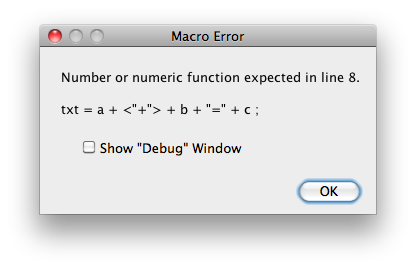
\includegraphics[scale=0.6]{fig/ErrorStringNumericFunction.png}
\caption{Error with Variable Assignment} \label{fig_ErrorVariable}
\end{center}
\end{figure}

This is because when ImageJ scans through the macro from top to bottom, line by line, 
it reaches the line for the assignment of the variable \ilcom{txt} and first sees the variable \ilcom{a} and interprets that \ilcom{txt} should be a numerical variable 
(or function), since \ilcom{a} is known to be a number as it was defined so in one of the lines above. Then ImageJ goes on interpreting rightward thinking that this is math. Then finding a "+" which surprisingly is a character
ImageJ cannot interpret string variable within a numerical function, so it returns an error message. The macro aborts.  

To overcome this problem, the programmer can tell ImageJ that 
\textit{txt} is a string function at the beginning of the assignment 
by putting a set of double quote. This tells the interpreter that this assignment is a string concatenation assignment and not a numerical assignment. 
ImageJ does handle numerical values within string function, 
so the line is interpreted without problem and prints out the result successfully. Note that such confusion of string and numerical types are rarely seen in general scripting languages and specific to ImageJ macro language.

\begin{indentexercise}{2}
Modify the code 4, so that the calculation involves subtraction (-), multiplication (*) and division (/). 
\end{indentexercise}